
\documentclass[runningheads]{llncs}

\usepackage{natbib}
\usepackage{mathptmx}
\usepackage[utf8]{inputenc}
\usepackage{amsmath}
\usepackage{amsfonts}
\usepackage{amssymb}
\usepackage[dvips,dvipdfm,pdftex]{graphicx}
\usepackage{pgfplotstable}
\usepackage{pgfplots}
\pgfplotsset{compat=newest}
\usepackage{array}
\usepackage{booktabs}
\usepackage{morefloats}
\usepackage{etex}
\usepackage{listings}
\usepackage{float}
\usepackage{epstopdf}
\usepackage[section]{placeins}
\usepackage[ruled,linesnumbered,resetcount,algochapter]{algorithm2e}
\usepackage{caption}
\captionsetup[table]{justification=raggedright, font=small, labelfont=bf, skip=5pt}

\begin{document}

\title{Open-set Web Genre Identification Using Distributional Features and Nearest Neighbors Distance Ratio}

\author{Dimitrios Pritsos \and Efstathios Stamatatos }

\institute{ University of the Aegean\\
            Karlovassi, Samos \textendash{} 83200, Greece.\\
            \email{\{dpritsos,stamatatos\}@aegean.gr}
}

\maketitle

\begin{abstract}
Web genre identification can enhance information retrieval systems by providing rich descriptions of documents and enabling more specialized queries. The open-set scenario is more realistic for this task since web genres evolve in time and it is not feasible to define a universally agreed genre palette. In this paper, we propose a novel approach based on distributional features acquired by doc2vec and a recently-proposed open-set classification algorithm, nearest neighbors distance ratio. We present experimental results using a benchmark corpus and a strong baseline and demonstrate that the proposed approach is competitive especially when emphasis is given on precision.

\keywords{Web genre identification \and Open-set classification \and Distributional features}
\end{abstract}


\section{Introduction}\label{sec:intro}

%Web Genre Identification (WGI) concerns the association of web pages with labels that correspond to their form, communicative purpose and style rather than their content. The ability to %automatically recognize the genre of web documents can enhance modern information retrieval systems by enabling genre-based grouping/filtering of search results or building intuitive %hierarchies of web page collections combining topic and genre information \citep{Braslavski2007,Rosso2008,de2009genre}. For example, a search engine can provide its users with the option %to define complex queries (e.g., blogs about machine learning or eshops about sports equipment) as well as the option to navigate through results based on genre labels (e.g. social media %pages, web shops, discussion forum, blogs, etc). The recognition of web genre can also enhance the effectiveness of processing the content of web pages in information extraction %applications. For example, given that a set of web pages has to be part-of-speech tagged, appropriate models can be applied to each web page according to their genre %\citep{Nooralahzadeh2014}. However, research in WGI is relatively limited due to fundamental difficulties emanating from the genre notion itself.
%
%The most significant difficulties in the WGI domain are: (1) There is not a consensus on the exact definition of genre \citep{crowston2011problems}; (2) There is not a common genre %palette that comprises all available genres and sub-genres \citep{santini2011cross,mehler2010genres_on_web,mason2009n,sharoff2010web}, moreover, genres are evolving in time since new %genres are born or existing genres are modified \citep{Boese2005}; (3) It is not clear whether a whole web page should belong to a genre or sections of the same web page can belong to %different genres \citep{jebari2015combination,madjarov2015web}; (4) Style of documents is affected by both genre-related choices and author-related choices %\citep{petrenz2011stable,Sharroff2010}. As a result, it is hard to accurately distinguish between personal style characteristics and genre properties when style is quantified.
%
%Most previous studies in WGI consider the case where all web pages should belong to a predefined taxonomy of genres %\citep{Lim2005,santini2007automatic,kanaris2009learning,jebari2014pure_URL}. However, this naive assumption is not appropriate for most applications related with WGI. Since it is not %possible to construct a universal genre palette, there should always exist web pages that would not fall into any of the predefined genre labels. We call such web pages \textit{noise} %which also includes web documents where multiple genres (predefined or not) co-exist \citep{santini2011cross,levering2008using}. The vast majority of previous work in WGI avoid to examine %the problems arising from the presence of noise and as a result it is not possible to estimate the effectiveness of most existing WGI approaches in realistic conditions.
%
%To handle noise in WGI there are two options. First, to adopt the closed-set classification setup having one predefined category devoted to noise. Since this category would comprise all %web pages not belonging to the known genre labels, it would not be homogeneous. Moreover, this noise class would be much more greater with respect to the other genres causing class %imbalance problems. The second option is to adopt the open-set classification setting where it is possible for some web pages not to be classified into any of the predefined genre %categories \citep{pritsos2013open}. This setup avoids the problem of class imbalance caused by numerous noisy pages and also avoids the problem of handling a diverse and highly %heterogeneous class. On the other hand, open-set classification requires strong generalization with respect to the closed-set setup \citep{scheirer2013toward}.
%
%A great variety of features to quantify the stylistic choices related to genre have been proposed in previous work. These are mainly based on textual content (e.g., character and word %n-grams) \citep{mason2009distance,Sharroff2010} and form or structure of the web page (html tags, image count, links count, etc.) \citep{Lim2005,levering2008using}. Both sources of %information are useful and usually their combination enhances a WGI model \citep{kanaris2009learning}. However, features extracted from textual content are more robust since they do not %depend on technology or format used to create a web page and therefore they are more likely to remain stable in time.
%
%In this paper, we focus on the evaluation of WGI in realistic conditions where we assume that the given genre palette covers only a subset of existing genres. Any web documents that does %not fall into the predefined genre categories is considered as noise. To be able to handle noise, we adopt the open-set classification setup. In particular, we are testing two open-set %classification models, one based on \textit{One-Class Support Vector Machines} (OCSVM) and another based on \textit{Random Feature Subspacing Ensembles} (RFSE). Several text %representation schemes based on textual content are examined and we focus on the appropriate selection of parameter settings for each model. Using two benchmark corpora we perform a %systematic evaluation of WGI models when noise is either unstructured (the true genre of noisy pages is not available) or structured (the true genre of noisy pages is available). In order %to handle the latter case, we employ the openness test in WGI that provides a detailed view of performance for a varying number of known/unknown labels. This test has already been used in %visual object recognition \citep{scheirer2013toward} and it perfectly fits the WGI task.
%
%The rest of the paper is organized as follows. In section \ref{sec:previous_work}, previous work on WGI is described. Section \ref{sec:Ensembles_Description} analytically presents the %open-set classification models used in this study. In section \ref{sec:experimental_setup}, the  benchmark corpora and the setup of the conducted experiments are described while in %section \ref{sec:Experiments_Results} the results of the conducted experiments are presented. Finally, in section \ref{sec:conclusions} the main conclusions drawn from this study are %summarized and future work directions are discussed.
%
\section{Relevant Work}\label{sec:previous_work}

The utillity of the text genre identification (and/or classification) has been realised by the natural languiage processing community and others like jouranlsim historians. In addition the technology advances and the new sience inovations cased the attraction to the field where genre identification on known corpora like the Gutenberg Project has been toroughtly tested[SANT REF].

Althought, the tradistonal bag-of-words aproach had better result with XABoost or other technics been tested for over a decade on genre identificaion or/and particualru on WGI, distibutional feature models are early showing their advnatages over the TF-IDF (or TF alone) models[|REF].

Previous work in WGI (and text genre identification in general) follows a typical closed-set text categorization approach where, first, features are extracted from documents and, then, a classifier is built to distinguish between classes. Moreover, sofisticated machine learning algorithms have been mostly evaluated such as SVM. However, the simple approaches like k-means, nearest neigbhros, etc where given equal or higher scores in performace. Recently, there ensemble methods attraced attention due to the fact that they can increase singificantly the perfromance of these simple ML algorithms. Additionaly, other methods extending the ensembles methodology like Random Forests have been alo became popular[REF].

Great attection historicaly on WGI, is paid to the appropriate definition of features that are able to capture genre characteristics. The features of a text have three main outputs derived after its preprocessing, and particulatly for WGI. First is to separate the HTML tags and other web-application funcitonality from the pure textual information \citep{Lim2005,levering2008using}. Second is to separate the text starture elements such as the pages, the paragraphs, the sentences[REF]. Third is to define the terms-types, i.e. weather the smalest unit of the text would be character n-grams or word n-grams, part-of-speach histograms, etc \cite{kumari2014web,petrenz2011stable,mason2009n,sharoff2010web}.

Related to the first and the second step most of the work was focused there together with the combinaiton for several textual with HTML features and/or exploiting the hyperlink functionarlity of the web-pages and web-sites \citep{zhu2011enhance,abramson2012_URL,jebari2014pure_URL,priyatam2013don_URL,asheghi2014semi}.

Only very recently the distributional features has been tested in the Genre Identification field with some success. As we aware of this study is the first testing the effect of the distributional features on the WGI for the first time [REF]. 


%
%The majority of previous studies in WGI disregard the presence of noise. Santini \citep{santini2011cross} defines \textit{structured noise} as the collection of web pages belonging to %several genres. Such structured noise can be used as a negative class for training a binary classifier \citep{Vidulin2007}. However, it is highly unlikely that such a collection %represents the real distribution of pages on the web. On the other hand, \textit{unstructured noise} is a random collection of pages \citep{santini2011cross}. The effect of noise in WGI %was first studied in \citep{shepherd2004cybergenre,kennedy2005automatic} where predefined genres were personal, organizational, and corporate home pages while noise consisted of non-home %pages. However, the distribution of pages into these four categories was practically balanced, hence it was not realistic. Dong et al.\citep{dong2006binary} uses noise as the majority %class in an experiment where 190 instances from personal homepage, FAQ, and e-shop categories were used in combination with 600 noise pages. Similarly, Levering et al %\citep{levering2008using} uses about 200 instances for the predefined genres of store homepages, product lists, and product descriptions in combination with about 800 other pages (noise).
%
%Concerning the classification models involved in WGI studies, when a given genre taxonomy is utilized and there is no noise, then well-known machine learning models, like SVMs, decision %trees, neural networks, naive Bayes, Random Forests, etc. are used \citep{Lim2005,santini2007automatic,kanaris2009learning,jebari2015combination,sharoff2010web}. In case of presence of %noise, in a clustering framework described in \citep{kennedy2005automatic} one cluster is built for each predefined class and another cluster is built for the noise. However, the most %common approach to handle noise is to build binary classifiers where the positive class is based on a certain predefined category and the negative class is based on the concatenation of %all other predefined categories plus the noise \citep{kennedy2005automatic,dong2006binary,levering2008using}. Such a combination of binary classifiers can also be seen as a multi-label %and open-set classification model where a web page can belong to different genres and it is possible for one page not to belong to any of the predefined genres. More concrete open-set %classification models for WGI were presented in \citep{stubbe2007genre,pritsos2013open}. However, these models were only tested in noise-free corpora \citep{pritsos2015clef}. More %recently, Asheghi \citep{Asheghi2015} showed that it is much more challenging to perform WGI in the noisy web in comparison to noise-free corpora.

\section{Distributional Features Learning}\label{sec:Gensim}

In this study we are using the Doc2Vec out-of-the-box algorithm which is based on the there publications PUBA, PUBB, PUBC while the algorithm can be found at Gensim package \url{https://github.com/RaRe-Technologies/gensim}. In particular we have implemented a special module inside our package, specialized for HTML prepossessing, named \textit{Html2Vec} (see \url{https://github.com/dpritsos/html2vec}) where a whole corpus can be fed and matrix of \textit{Bag-of-Words Paragraph Vectors} (PV-BOW) is returned as an output. One PVBOW vector per Web-document for the corpus.

In order to compare our work to previews works, two different document representation types can be produced form our \textit{Gensim based sub-module}. One is PVBOW Word-n-grams and the other for PVBOW Character-n-grams, which are presented in our following experimental results.

The PVBOW is a \textit{Neural Network} (NNet) where it is formed as a \textit{softmax} multi-class classifier approximating the formula of eq.\ref{eq:softmax}. PVBOW is trained using \textit{stochastic gradient descent} where the gradient is obtained via \textit{back-propagation}. The objective function of the NNet is the maximized \textit{average log probability} eq.\ref{eq:objFN}, given a sequence of training n-grams (word of character) $t_{1}, t_{2}, t_{3}, ..., t_{T}$.

\begin{equation} \label{eq:objFN}
    \max{\frac{1}{T} \sum^{a=k}_{T-k}{\log{p(t_{a}|t_{a-k},...,t_{a+k})}}}
\end{equation}

\begin{equation} \label{eq:softmax}
    p(t_{a}|t_{a-k},...,t_{a+k}) = \frac{e^{y_{t_{a}}}}{\sum_{i}{e^{y_i}}}
\end{equation}

Particularly for PVBOW, we are using for this study, for each iteration, of the stochastic gradient descent, a \textit{text window} is sampled with size $w_{size}$. Then a random word is sample from the text window and \textit{form a classification task given the Paragraph Vector}. Thus the $y$ of the eq.\ref{eq:softmax} is formed to be $y = b + s(t_{1},t_{2},t_{3},...,t_{w_{size}})$ where $s()$ is the sequence of words-n-grams or character-n-grams of the sampled window.

In our study we are training a PVBOW Distributional Feature model for the whole corpus. The corpus initially is split to a set of paragraphs, as required from PVBOW. To be more specific the paragraphs are sentences split from all the document of the whole corpus. Then several models PVBOW feature models are trained for a variety of parameters and vector dimensions, explained in the experiments section below. After the model has been fitted then one vector for each web-document was inferred from the PVBOW. The final document vectors derived from \tetxit{Distributional Feature Model} are given to the open-set learning model explained below.

\section{Nearest Neighbors Distance Ratio}\label{sec:NNRD_Description}

The Nearest Neighbors Distance Ratio (NNRD) algorithm is our variant implementation of the proposed open-set algorithm of Mendes et al. \cite{mendesjunior2016}. In the original approach euclidean distance has been used because of the variation of data set on which the algorithm has been evaluated. In our approach we are using cosine distance, because in text classification is being confirmed to be the proper choice in hundreds of publications. Moreover, the cosine distance is comparable to the results of the \textit{Random Feature Sub-spacing Ensemble} algorithm found in \cite{pritsos2018open} where cosine similarity is used for the WGI evaluation.

The NNRD algorithm is an extension of the simple \textit{Nearest Neighbors} NN algorithm where additionally to the sets of training vectors (one set for each class) a threshold is selected by maximizing the \textit{Normalized Accuracy} (NA) as shown in equation\ref{eq:NA}) on the \textit{Known} and the \textit{Marked as Unknown samples}.

\begin{equation} \label{eq:NA}
    NA = \lambda A_{KS} + (1 - \lambda) A_{MUS}
\end{equation}

\noindent
where $A_{KS}$ is the \textit{Known Samples Accuracy} and $A_{MUS}$ is the \textit{Marked as Unknown Samples Accuracy}. The balance parameters \lambda regulates the mistakes trade-off on the known and marked-unknown samples prediction.

The optimally selected threshold is the the \textit{Distance Ratio Threshold} (DRT) where NA is maximized. Equation \ref{eq:DR} is used for calculating the Distance Ratio (DR) of the two nearest class samples, say $s_{c_{a}}$ and $u_{c_{b}}$, to a random sample $r_{x}$ under the constrain $c_{a} \notequal c_{b}$, where $c_{g}$ is the sample's class.

It is very important to note that the $c_{g}$ is trained in an open-set framework, therefore, the samples pairs selected for comparison might either be from the known of the marked as unknown samples. Thus $g \in {1,2,...,N}$ and $g = \emptyset$ when samples is marked as unknown.

\begin{equation} \label{eq:DR}
    DR = \frac{D(r_{x}, s_{c_{a}})}{D(r_{x}, s_{c_{b}})}
\end{equation}
\noindent
where $D(x,y)$ is the distance between the samples where in this study is the \textit{Cosine Distance}.

Therefore, the fitting function of the NN algorithm, described in pseudo-code \ref{alg:NNDR_fitting}, is the optimization procedure to find the DRT values for classes respective sets of training samples where NA is maximized.

\hfill \break

\begin{algorithm}[H]
\caption{\textit{Nearest Neighbor Distance Ratio} training data fitting function}\label{alg:NNDR_fitting}
\KwData{$G$ the set of genre class tags $\{1,2,...,N\}$,
        $p$ the hyper-parameter regulates the percentage of $G$ tags will be marked as unknown,
        $k$ the hyper-parameter regulates the percentage of known $G$ tags that will be keept for validation only,
        $T$ the \textit{Distance Ratio} thresholds set than will test for finding the one which is minimizing the \textit{Normalized Accuracy},
        $\lambda$ regulates the mistakes trade-off on the known and marked-unknown samples prediction (see eq.\ref{eq:DR}),
        $C[g]$ the matrix of class vector sets one for every genre class tag $g \in G$}
\KwResult{$DRT$ the \textit{Distance Ration Threshold} calculated by the NNRD algorithm's fitting function, $C[g]$}

$K^{G}_i, K^{G}_{validation}_i, U^{G}_{validation}_i, I^{G} = Split(G,p,k)$ splitting the $G$ tags in to known/unknown samples combinations using the $p$ and $k$ hyper-parameters. The amount of split combinations is calculated by the equations \ref{eq:splt_percent} and \ref{eq:splt}.\;

$V^{G} = U^{G}_{validation} \cup K^{G}_{validation}$ the validation set is the union of the $I$ splits of the known-validation and the marked-as-unknown sets, of the whole training set\;

\For{each $i \in I$}{
    $D^{cos}_{VK}[i] = COS_{D}(V^{G}_i, K^{G}_i)$ calculating all the Cosine Distances between the web-page of $K^{G}$ and $V^{G}$ sets for \textit{every $I$ split combination};
}

$Ci^{min}_{A} = argmin(D^{cos}_{VK})$ getting the indices of the closest classes from $V$\;
$Ci^{min}_{B} = argmin(D^{cos}_{VK})$ getting the indices of the \textit{second closest} classes from $V$\;

$R_{V} = D^{cos}_{VK}[Di^{min}_{A}] / D^{cos}_{VK}[Di^{min}_{B}]$ calculating the Distance Rations $R$ for all the vectors in $V$

$NA^{max} \gets 0$ initializing \textit{Maximized Normalized Accuracy} with $0$ value.
$DRT \gets 0$ initializing \textit{Distance Ratio Threshold} with $0$ value.

\For{each $drt \in T$}{

    \For{each $r, i \in \{R_{V}, count(R_{V})\}$}{

        \eIf{$r < drt$}{
            $vi = Ci^{min}_{A}[i]$ keep the respective index\;
            $Y[i] = G[vi]$ setting the genre's class tag as prediction for this random vector of set $V$\;
        }
        {
            $Y[i] = \emptyset$ setting as none of the known genres or "I don't know"\;
        }

    }

    $NA_{V} = NormalizedAccuracy(Y, R_{V})$ calculating the Normalized Accuracy as shown in equation \ref{eq:NA} for tested threshold $drt$\;

    \eIf{$NA_{V} > NA^{max}$}{
        $NA^{max} \gets NA_{V}$ keeping the maximum $NA$ until the outer for-loop finishes\;
        $DRT \gets drt$ keeping the \textit{Distance Ratio Threshold} maximizes the \textit{Normalized Accuracy}\;
    }

}

\end{algorithm}

In the optimization procedure the training samples are split based on their class tags $c_{x}$. Then some class tags are \textit{marked as unknown} and some are left being known. Therefore, all the samples of the marked as unknown are used only in the validation subset while the known class tags samples are farther split into the classes sets (one for each class) and into the known validation set. Then, samples of the validation sets, both then known and then marked as unknown, are used seamlessly for calculating the set of Distance Rations (one for each class). Afterwards, a set of DRT values are tested given a range of values $R \in {t_{1}, t_{2}, t_{n}}$ beforehand where the $t_{x}$ is selected which is maximizing the NA of the validation set.

The splitting procedure the of the training set is regulated by a hyper-parameter $p$ which defines the percentage of the class tags set $g \in {1,2,...,N}$ where they will be marked as unknown. Then the total number of all possible splitting combination are calculated and these split-sets are used for finding the DRT. The combination are found using equations \ref{eq:splt_percent} and \ref{eq:splt}, where eq.\ref{eq:splt} is the \textit{Binomial Coefficient}.

\begin{equation} \label{eq:splt_percent}
    U_{num} = int(N * p)
\end{equation}

\noindent
where $N$ is the size of the class tags set ${1,2,...,N}$ and $p$ is the percentage regulation parameter for keeping the number of tags to be marked as unknown.

\begin{equation} \label{eq:splt}
    S_{num} = \frac{N!}{U_{num}!(N-U_{num})!}
\end{equation}

The NNDR is a open-set classification algorithm, therefore, every random sample will be classified to one of the classes the NNRD has been fitted or to the unknown when its DR is greater then DRT. While training as explained above the DRT values are tested incrementally until the optimal data fitting for the training function.

In prediction phase the DRT is passed to the NNDR prediction function together with the random samples and the training samples as shown in pseudo-code \ref{alg:NNDR_prediction}.

\begin{algorithm}[H]
\caption{\textit{Nearest Neighbor Distance Ratio} prediction function}\label{alg:NNDR_prediction}
\KwData{ $W$ the vector set of the random web-page to be classified,
         $C[g]$ the matrix of class vector sets one for every genre class tag $g \in G$,
		 $DRT$ the \textit{Distance Ration Threshold} calculated by the NNRD algorithms fitting function}
\KwResult{ $Y \in \{G,\,\emptyset\}$,
           $R$ the Distance Ratio scores vector, one score for every input vector of the random set $W$}

\For{each $g \in G$}{
    $D^{cos}_{C_{g}X} = COS_{D}(C[g], X)$ calculating all the Cosine Distances between the random web-page vectors and the class vectors of class $g$\;
}

$Ci^{min}_{A} = argmin(D^{cos}_{C_{g}W})$ getting the indices of the closest classes from $W$\;
$Ci^{min}_{B} = argmin(D^{cos}_{C_{g}W})$ getting the indices of the \textit{second closest} classes from $W$\;

$R_{W} = D^{cos}_{C_{g}W}[Di^{min}_{A}] / D^{cos}_{C_{g}W}[Di^{min}_{B}]$ calculating the Distance Rations $R$ for all the vectors in $W$

\For{each $r, i \in \{R_{W}, count(R_{W})\}$}{

    \eIf{$r < DRT$}{
        $vi = Ci^{min}_{A}[i]$ keep the respective index\;
        $Y[i] = G[vi]$ setting the genre's class tag as prediction for this random vector of set $W$\;
    }
    {
        $Y[i] = \emptyset$ setting as none of the known genres or "I don't know"\;
    }

}

\end{algorithm}

Our implementation of the above NNRD algorithm can be found at \url{https://github.com/dpritsos/OpenNNDR}, where it is implemented in Python/Cython and can significantly accelerated using as much as possible CPUs due to its capability for concurrent calculations in C level speed. Since, NNRD is a rather slow classification method, we have seen in practice that there is up to 100 time acceleration from the capability to exploit a cloud service with 32 vCPUs (Xeon) compare to 4-core/8-threads i7 CPU.

\section{Experiments}\label{sec:experimental_setup}

\subsection{Open-set Evaluation Methodology}
In this study we are measuring the performance of a novel extension of the NN method, designed for open-set classification when the web-documents used as input are \textit{Distributional Encoding of Fixed Size Vectors} derived from an PVBOW NNet model. In particular we are measuring the effect the marked-as-unknown (or marked-as-noise) genre class tags, to the open-set prediction process.

To compensate the potentially unbalanced distribution of web pages over the genres, we are using the macro-averaged precision and recall measures. Than is a modified version of precision and recall for open-set classification tasks proposed by \cite{mendesjunior2016}. This modification calculates precision and recall only for the known classes (available in the training phase) while the unknown samples (belonging to classes not available during training) affect false positives and false negatives. To find parameter settings that obtain optimal evaluation performances we use two scalar measures, the \textit{Area Under the Precision-Recall Curve} (AUC)and $F_{1}$. We will show that the appropriate selection of the optimization measure is highly significant in the presence of noise.

Precision-Recall curve is a standard method to visualize the performance of classifiers. In this paper, the Precision-Recall curve is calculated in 11-standard recall levels $[0,0.1,...,1.0]$. Precision values are interpolated based on the following formula:

\begin{equation}
	P(r_j)=max_{r_j \leqslant r \leqslant r_{j+1}}(P(r))
\end{equation}

\noindent
where $P(r_j)$ is the precision at $r_j$ standard recall level.

\subsection{Corpora}\label{sec:corpora}
In this paper we study NNRD performance with distributional features derived from a NNet PVBOW corpus. In particular, the open-set algorithms described above are analytically tested on benchmark corpus already used in previous work in WGI \citep{meyer2004genre,santini2007automatic,kanaris2009learning,pritsos2018open}, the \textit{SANTINIS} \cite{mehler2010genres_on_web} corpus.Details are given in table \ref{tbl:genre_tags}. This is a corpus comprising 1,400 English web pages evenly distributed into 7 genres as well as 80 BBC web pages evenly categorized into 4 additional genres. In addition, it comprises a random selection of 1,000 English web pages taken from the SPIRIT corpus \cite{joho2004spirit}. The latter can be viewed as noise in this corpus. In particular in this study SPIRIT tags are considered \textit{Marked as Unknown} (MU) and this is how we measure them.

Note that in the evaluation process we both measuring two kind classification-as-unknown of the open-set algorithm; the \textit{false positive unknown} where are classification of samples which have class tags known to the NNRD model and the \textit{true positive unknown} where they are marked-as-unknown (or marked-as-noise) where they are considered as noise.

\subsection{Settings}\label{sec:evaluation_measures}
Our text representation features are based exclusively on textual information from web pages excluding any structural information, URLs, etc. Based on the good results reported in \citep{sharoff2010web,pritsos2013open,Asheghi2015} as well as some preliminary experiments. The following document representation schemes are examined: Character 4-grams (C4G), Word unigrams (W1G), and Word 3-grams (W3G).

We use the Term-Frequency (TF) weighting scheme and Distributional Learning scheme. The feature space for TF is defined by a \textit{Vocabulary} which is extracted based on the terms appearing at training set only. The TF-Vocabulary range of dimensions have been tested are $V_{TF}\textit{=\{5k,10k,50k,100k\}}$. The feature space in the Distributional model is pre-selected while the deep learning process of PVBOW model. The range of the models fixed dimensions has been tested are $D_{dim}\textit{=\{50,100,250,500,1000\}}$ based of previews studies related to the distributional features on Natural Language Processing domain where relatively small dimensions are used, compare to TF scheme.

The DM vocabulary creation process is also driven by an internal terms \textit{vocabulary} which is used for eliminating the terms with lower than a preferred frequency and then discards the terms from the text window for the PVBOW (see section \ref{sec:Gensim}). In this study we have tested as the $TF_{min}=\{3,10\}$ minimum frequencies set. The text window tested was $P_{win}=\{3,8,20\}$ size set. In respect of PVBOW model, other (hyper-)parameter values put to a test were $\alpha=0.025$, $epochs=\{1, 3, 10\}$ and $decay=\{0.002, 0.02\}$.

Particularly for NNRD then following parameters have been tested:1) $\lamba\textit{=\{0.2, 0.5, 0.7\}}$ which is regulating the balance between the known and the unknown classification accuracy risk in the formula \ref{eq:NA}, 2)DRT threshold selection candidates $DRT\textit{=\{0.4, 0.6, 0.8, 0.9\}}$. Also two other parameters we have introduced in our implementation; the percentage of the training set to be split internally as Training/Validation sub-sets where $V_{ptg}\textit{=\{0.5, 0.7\}}$ has been tested. Then the percentage of the validation set which was split as unknown $U_{ptg}\textit{=\{0.3, 0.5\}}$ has been tested.

%The Random Feature Sub-spacing Ensemble (RFSE) algorithm is a variation of the method presented by Koppel et al. \citep{koppel2011authorship} for the task of \textit{author identification}. In the original %approach, there is only one training example for each author and a number of simple classifiers is learned based on random feature subspacing. Each classifier uses the cosine distance to estimate the most %likely author. The key idea is that it is more likely for the true author to be selected by the majority of the classifiers since the used subset of features will still be able to reveal that high similarity. %That is, the style of the author is captured by many different features so a subset of them will also contain enough stylistic information. Since WGI is also a style-based text categorization task, this idea %should also work for it.
%
%In our study we adopt the RFSE method as introduced in \citep{pritsos2013open} shown in \textit{Algorithm \ref{alg:RFS-Ensemble}}. There are multiple training examples (documents) for each available genre. To %maintain simplicity of classifiers, we have used a \textit{centroid vector} for each genre. In the training phase, a centroid vector is formed, for every class, by averaging all the Term-Frequency (TF) vectors %of the training examples of web pages for each genre.
%
%The class centroids are all formed for a given feature type. Then, an evaluation document is compared against every centroid and this process is repeated $I$ times. Every time a different feature sub-set is %used. Then, the scores are ranked from highest to lowest and we measure the number of times the document is top-matched with every class. The document is assigned to the genre with maximum number of matches %given that this score exceed a predefined $\sigma$ threshold. In the opposite case, the document remains unclassified, the RFSE responds "I Don't Know".

As comparative \textit{Baseline} we have employed RFSE. With respect to RFSE, four parameters should be set: the vocabulary size $V_{F}$, the number of features used in each iteration $FSS$, the number of iterations \textit{I}, and the threshold $\sigma$. We examined, $FSS$=\textit{\{1k, 5k, 10k, 50k, 90k\}}, \textit{I}=\textit{\{10, 50, 100, 200, 300, 500, 1000\}} and $\sigma$\textit{=\{0.5, 0.7, 0.9\}}. Additionally, in this work we are testing three document similarity measures: cosine similarity. All these parameters have been selected as suggested in \cite{pritsos2018open}.

Finally, to extract the best possible parameter settings for each classification method we apply grid-search over the space of all parameter value combinations.

\begin{table}
\center
\begin{tabular}{|l|l|}
\hline
\multicolumn{1}{|c|}{Genre} & \multicolumn{1}{c|}{Pages} \\
\hline
\multicolumn{1}{|l|}{Blog} & \multicolumn{1}{c|}{200}  \\
\multicolumn{1}{|l|}{Eshop} & \multicolumn{1}{c|}{200} \\
\multicolumn{1}{|l|}{FAQ} & \multicolumn{1}{c|}{200} \\
\multicolumn{1}{|l|}{Frontpage} & \multicolumn{1}{c|}{200} \\
\multicolumn{1}{|l|}{Listing} & \multicolumn{1}{c|}{200} \\
\multicolumn{1}{|l|}{Personal Home Page} & \multicolumn{1}{c|}{200} \\
\multicolumn{1}{|l|}{Search Page} & \multicolumn{1}{c|}{200} \\
\multicolumn{1}{|l|}{DIY Mini Guide (BBC)} & \multicolumn{1}{c|}{20} \\
\multicolumn{1}{|l|}{Editorial (BBC)} & \multicolumn{1}{c|}{20} \\
\multicolumn{1}{|l|}{Features (BBC)} & \multicolumn{1}{c|}{20} \\
\multicolumn{1}{|l|}{Short Bio (BBC)} & \multicolumn{1}{c|}{20} \\
\multicolumn{1}{|l|}{Noise (Spirit1000)} & \multicolumn{1}{c|}{1000}  \\
\hline
\end{tabular}
\caption {SANTINIS corpora descriptions and amount of pages per genre.}
\label{tbl:genre_tags}
\end{table}


\section{Results}\label{sec:Experiments_Results}

In this study we are evaluating the performance of NNDR algorithm into the open-set framework with the presence of noise, as the notion of noise explained above. That is we are only using the 11 known genre classes of SANTINIS corpus for training, while for evaluation we are using all 12 classes. The true genre class tags for the documents of the in the 12th class is not known and it is only considered as noise. Therefore, we have to deal with \textit{unstructured noise}. Additionally, since the noise-class is marked then the algorithm is evaluated in both false-positive classifications of the marked-unknown-classes as known an the false-negative classifications of the known-classes as unknown. In both cases the false classifications are causing a penalty to the Macro-F1 and Macro-Precision-Recall Curves we are using for evaluation.

We perform  10-fold cross validation and in each fold we include the full set of 1,000 pages of noise. This evaluation strategy is giving a more realistic evaluation. Since the noise size is greater than the size of any genre included in the given genres collection.

Initially we are comparing the performance of NNDR with RFSE on TF features vocabulary. RFSE returns higher score to NNDR, in tables \ref{tbl:NNDR_TF} and \ref{tbl:RFSE_TF}, for Macro-F1 and Macro-AUC and for any terms-type. Note also that the TF feature model dimensions for both algorithm is in all cases a few thousands.

\pagebreak

\begin{table}
\center
\begin{tabular}{|l|cccc|lr|rrrr|}
\hline
MAX. & STP & SUP & DRT & $\lambda$ & T.TYPE & DIMs & M\emph{P} & M\emph{R} & M\emph{AUC} & M\emph{F1} \\
\hline
F1 & 0.7 & 0.3 & 0.8 & any & C4G & 5000 & 0.664 & 0.403 & 0.291D & 0.502 \\
AUC & 0.7 & 0.3 & 0.8 & any & C4G & 5000 & 0.664 & 0.403 & 0.291D & 0.502 \\
F1 & 0.7 & 0.5 & 0.8 & any & W1G & 5000 & 0.691 & 0.439 & 0.348D & 0.537 \\
AUC & 0.7 & 0.5 & 0.8 & any & W1G & 5000 & 0.691 & 0.439 & 0.348D & 0.537 \\
F1 & 0.5 & 0.5 & 0.8 & 0.3 or 1.5 & W3G & 10000 & 0.720 & 0.664 & 0.486D & 0.691 \\
AUC & 0.5 & 0.5 & 0.6 & 0.5 & W3G & 5000 & 0.738 & 0.604 & 0.437D & 0.664 \\
\hline
\end{tabular}
\caption {Maximum performance of NNDR on TF Features of SANTINIS coprus. STP is the Spliting Training Percentage. SUP is the Splitting Unknown Percentage. DRT is the Distance Ration Threshold. $\lambda$ is the weigthing balance regulation parameters for the Normalized Accuracy. T.TYPE is the Terms Type. DIMs is the features model's dimensions. MP is the Macro Precision. MR is the Macro Recall. MAUC is the Area Under the Macro PR Curve. MF1 is the F1 score of the Macro Precision and Macro Recall.}
\label{tbl:NNDR_TF}
\vspace{-15mm}
\end{table}

\begin{table}
\center
\begin{tabular}{|l|ccc|lr|rrrr|}
\hline
MAX. & FSS & $\sigma$T & ITER. & T.TYPE & DIMs & M\emph{P} & M\emph{R} & M\emph{AUC} & M\emph{F1} \\
\hline
F1 & 1000 & 0.5 & 100 & C4G & 50000 & 0.739 & 0.780 & 0.652 & 0.759 \\
AUC & 500 & 0.5 & 300 & C4G & 10000 & 0.686 & 0.831 & 0.722 & 0.751 \\
F1 & 10000 & 0.5 & 1000 & W1G & 50000 & 0.776 & 0.758 & 0.657 & 0.767 \\
AUC & 1000 & 0.5 & 300 & W1G & 5000 & 0.618 & 0.807 & 0.673 & 0.700 \\
F1 & 1000 & 0.7 & 100 & W3G & 50000 & 0.797 & 0.722 & 0.488 & 0.758 \\
AUC & 10000 & 0.5 & 100 & W3G & 100000 & 0.657 & 0.805 & 0.696 & 0.723 \\
\hline
\end{tabular}
\caption {Maximum performance of RFSE on TF Features of SANTINIS coprus. FSS is the Features Subset Selection number. $\sigma$T is the sigma threshold of the RFSE. ITER is the number of iterations of the RFSE. T.TYPE is the Terms Type. DIMs is the features model's dimensions. MP is the Macro Precision. MR is the Macro Recall. MAUC is the Area Under the Macro Precision-Recall Curve. MF1 is the F1 score of the Macro Precision and Macro Recall.}
\label{tbl:RFSE_TF}
\vspace{-15mm}
\end{table}

\begin{table}
\center
\begin{tabular}{|l|cccc|lr|ccccr|rrrr|}
\hline
MAX. & STP & SUP & DRT & $\lambda$ & T.TYPE & DIMs & MTF & WS & $\alpha$ & EP. & DEC. & M\emph{P} & M\emph{R} & M\emph{AUC} & M\emph{F1} \\
\hline
F1 & any & any & 0.8 & any & C4G & 50 & 3 & 8 & 0.025 & 10 & 0.002 & 0.829 & 0.600 & 0.455D & 0.696 \\
AUC & any & any & 0.8 & any & C4G & 500 & 3 & 3 & 0.025 & 10 & 0.02 & 0.755 & 0.602 & 0.539D & 0.670 \\
F1 & any & any & 0.8 & any & W1G & 50 & 3 & 3 & 0.025 & 10 & 0.02 & 0.733 & 0.670 & 0.541D & 0.700 \\
AUC & any & any & 0.8 & any & W1G & 50 & 3 & 3 & 0.025 & 10 & 0.02 & 0.733 & 0.670 & 0.541D & 0.700 \\
F1 & any & any & 0.8 & any & W3G & 100 & 3 & 3 & 0.025 & 10 & 0.02 & 0.827 & 0.615 & 0.564D & 0.706 \\
AUC & any & any & 0.8 & any & W3G & 100 & 3 & 3 & 0.025 & 10 & 0.02 & 0.827 & 0.615 & 0.564D & 0.706 \\
\hline
\end{tabular}
\caption {Maximum performance of NNDR on Distributional Features of SANTINIS corpus. STP, SUP, DRT, $\lambda$, T.TYPE, DIMs are the same as in table \ref{tbl:NNDR_TF}. MTF is the Minimum Threshold Fequency of the Distributional models Vocabulary. WS is the Windows Size of the text sentence. $\alpha$ is the NNet parameter. EP is the epochs number of the NNet model. DEC is the decay parameter of the NNet model. MP is the Macro Precision. MR is the Macro Recall. MAUC is the Area Under the Macro PR Curve. MF1 is the F1 score of the Macro Precision and Macro Recall.}
\label{tbl:NNDR_Gensim}
\vspace{-20mm}
\end{table}

\pagebreak


However, there is a notable difference in the behavior of the two algorithms where it seems to be the reason RFSE outperforms NNDR. NNDR is using the 5000 (with the exception of line 4 of table \ref{tbl:RFSE_TF}) most frequent features for both training and evaluation phases. RFSE is using about 1000 \textit{randomly selected features} from the 50,000 to 100,000 most frequent features. This observations leading as the conclusion that the textual-genre information is pervasive in several features of the texts irrespectively of their frequency.

In order to research our null hypothesis where the textual-genre information is pervasive in the correlation of the features and not only in their frequency, we employee the distributional features explained above. Comparing tables \ref{tbl:NNDR_TF} and \ref{tbl:NNDR_Gensim} there is a notable improvement. Particularly for the Macro-F1 Score the performance reaches $0.7$ in all cases. Moreover, the STP, SUP and $\lambda$ parameters can my any of the set we have tested, on the contrary to the TF features model where only a specific value pare case is returning the maximum performance. Concerning TF model only when W3G terms-type is used we have a comparable $F1$ and $AUC$ value to the respective performance of the distributional model for NNDR.

We have also examined the case where $AUC$ is maximized because it seems in \cite{pritsos2018open} study this measure is maximized when precision is maximized while the recall is kept as max as possible. As an example note line 6 at table \ref{tbl:NNDR_TF} where for W3G the precision can reach $0.738$ while recall only reduced to $0.604$ compare to the $0.664$ in the above line where F1 is maximized.

The open-set classification framework evaluation design naturally turns our interest to the precision performance of the algorithms. To reason it we have to consider that a classifier in a binary case should distinguish the \textit{known and the unknown web documents} are not belonging to the target class. In addition it has to recognize the the documents of the target class. Thus 2 out of 3 evaluation score naturally related to the precision score.

In precision perspective it seems NNDR with distributional features outperforms RFSE in all case. In addition the size of features models dimension are 10 to 200 times smaller. NNDR returns $0.829$ macro-precision score compare to $0.739$ of the RFSE, for C4G terms-type. Moreover, the maximum precision of RFSE is $0.797$ with $0.722$ recall while the respective recall for them maximum NNDR precision performance is $0.600$.

The performance of NNDR (with distributional features) increases for $10\%$ on average for precision and decreases for $21.00\%$ compare to the RFSE. In addition, its performance increases for $7\%$ in precision and $37\%$ in recall compare to it self when TF feature model is used.

We further evaluated the performance of NNDR in respect of precision performance and for this reason we have selected the best performance with the AUC criterion for NNDR using DF model, which in for this corpus is also maximizes $F1$. In figure \ref{fig:NNDR_W3G_Best_RFSE_Baseline} NNDR with DF, NNDR with TF and RFSE with TF are shown. All curves are showing the performance when W3G is used where it the case NNDR with DF is returning the maximum performance on SANTINIS corpus.

\begin{figure}[H]
\begin{center}
    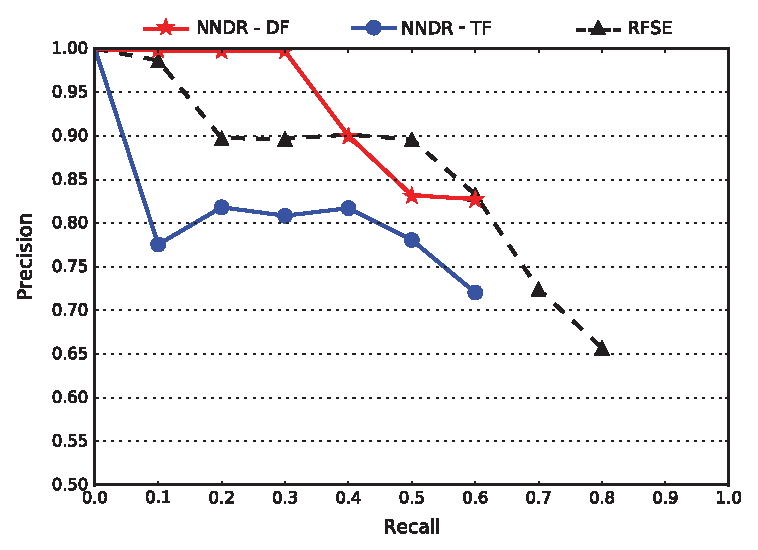
\includegraphics[scale=0.99]{NNDR_W3G_Best_RFSE-Baseline_2.eps}
	\caption{Precision-Recall Curves of NNDR on SANTINIS corpus with RFSE as Baseline. The curves are for W3G terms-type and for AUC optimization criterion. The 11-recall-levels are shown for each evaluation experiment. The lines are stopping before the 11th recall level due to the open-set framework, i.e. the remaining part after the last mark of each curve it the percentage of the corpus tha has been classified as Unknown from the algorithms.}
	\label{fig:NNDR_W3G_Best_RFSE_Baseline}
	\end{center}
\end{figure}

The NNDR-DF is starting higher from all the curves and it remains to $0.99$ precision for the $30\%$ of the corpus then it drops to the same level with the RFSE baseline and after $0.50\%$ drops below it. However, it remains over $0.80$ up to $60\%$ of the corpus. The the rest of the corpus is classified as unknown. RFSE manages to recognize correctly part of the corpus up to $80\%$ with the precision to drop to $0.70$ and then to $0.65$. Considering the NNDR-TF is significantly lower in performance compare to the base line and is also has a significant drop in performance for the first $10\%$ of the corpus. Given that the curves are calculated based on the ranked scores from the best performance to the lowest performance it seems that the algorithm significantly affected by the noise of the marked-unknown part. That is the algorithm makes very confident decision for some part of the corpus confusing them with other classes. Its overall performance is over $0.7$ precision and still recognize the $60\%$ of the corpus.

To conclude it seems that distributional features are giving a significant increment in performance even for a pure performance and very algorithm as NN, particularly the NNDR, i.e. an open-set version of it. Still RFSE where has successfully used for  WGI and other NLP problems, is giving higher over all performance in respect of macro-F1 and AUC. However, in respect of precision which is naturally more important for an open-set evaluation set the distributional features are offering higher or equal performance with 100 times smaller feature size. Moreover, considering the open-set framework as a filtering-setup for the algorithms one would probably prefer the NNDR-DF algorithm over RFSE.



\section{Conclusions}\label{sec:conclusions}

In this paper we presented an experimental study where is focused on the effect of distributional features on an open-set web-page document classification task. In contrast to vast majority of previous work in this area, we adopt the open-set scenario that is more realistic for  web-page classification since it is not feasible to construct a genre palette with all available genres and appropriate samples for each one of them. Particularly we are evaluating the possible performance improvement of an open-set algorithm when distributional features are employed, using the SANTINIS corpus.

The open-set algorithm we have evaluated with distributional features input is a novel variation of Nearest Neighbors algorithm named NNDR. A Distance Ration threshold is calculated while the training procedure for maximizing the \textit{Normilized Accuracy} of the known and the unknown classes.

Our evaluation methodology previews shown to be proper for evaluation open-set scenarios. The natural focus in an open-set evaluation framework is the macro-precision, since always there is a part of the corpus will be classified as unknown. Either because it is unknown (marked-as-unknown) or it is considered as outage while training.

In our evaluation distributional feature are giving a great improvement to the NNDR algorithm compare to it TF features performance. Moreover comparing it to the RFSE algorithm, our baseline, there is also an improvement in respect of macro-precision with some cost to the recall performance. Overall NNDR from a very low performance compare to the baseline it is becoming a comparable choice.

As concerns the terms-types, either fo the TF features model of the distributional one in all cases W3G provided the maximum scores.
distributional
In this study we concluded that probably the distributional features is a prospective choice for the WGI research community. Thus, a farther research would be fruitful focusing on several important aspects the selection of the similarity measures other than cosine we have used. There are also several variation and parameters for the distributional features one can use, for instance we have used Bag-of-words-paragraph vectors for training on our NNet deep learning model.

Finally it almost became tradition to be underlined that there is a need for a well formed corpus specialized for the WGI task. We need larger corpora including multiple genre labels. In addition there is a need for a constant updating of this corpus to capture the new trends in the genre pallet of the web itself, since new genre classes are added and the current ones are rapidly changing context, as naturally the human communication is reformed in a temporal manner.

\bibliographystyle{splncs04}
\bibliography{ECIR2019}

\end{document}
